\documentclass[a4paper,12pt]{article}
\usepackage[utf8]{inputenc}
\usepackage[russian]{babel}
\usepackage{amsmath, amssymb}
\usepackage[hyperfootnotes=false]{hyperref}
\usepackage{geometry}
\usepackage{indentfirst}
\usepackage{graphicx}
\usepackage{float}
\usepackage{enumitem}
\usepackage{caption}
\usepackage{array}
\geometry{
	a4paper,
	top=24mm,
	bottom=30mm,
	left=20mm,
	right=20mm
}

\newcommand{\blfootnote}[1]{%
	\begingroup
	\renewcommand{\thefootnote}{}%
	\footnote{#1}%
	\addtocounter{footnote}{-1}%
	\endgroup
}

% Отступ первой строки абзаца 1 см
\setlength{\parindent}{1cm}
\setlength{\parskip}{0pt}
\linespread{1}                 % одинарный интервал

% Отключение нумерации страниц
\pagenumbering{gobble}

% Настройка подписей рисунков и таблиц
% Используем \caption* для отключения точки, но оставляем обычный \caption
\usepackage[labelsep=space, justification=centering]{caption}
\captionsetup[figure]{font=small}   % small = 11pt при 12pt основного шрифта
\captionsetup[table]{font=small}
\renewcommand{\figurename}{Рис.}
\renewcommand{\tablename}{Табл.}

% Убираем точку в конце подписи (переопределяем \caption)
\usepackage{etoolbox}
\makeatletter
\renewcommand{\fnum@figure}{\figurename~\thefigure}
\renewcommand{\fnum@table}{\tablename~\thetable}
\apptocmd{\@caption}{\def\@captionheadfont{\normalfont}\def\@captionfont{\normalfont}}{}{}
\makeatother

% Настройка списка литературы
\makeatletter
\renewcommand{\@biblabel}[1]{#1.}   % нумерация "1.", "2."
\makeatother

\begin{document}
	
	\noindent УДК 621.373.826:536.24
	
	\begin{flushright}
		И. М. Куликовских$^{1}$\blfootnote{*) И. М. Куликовских, kulikovskih.im@edu.spbstu.ru}, Г. О. Корнышов$^{2}$
	\end{flushright}
	
	
	\begin{flushright}
		$^{1}$Санкт-Петербургский политехнический университет Петра Великого\\
		$^{2}$Физико-технический институт им. А.Ф. Иоффе РАН
	\end{flushright}
 	
	\vspace{12pt}
	
	\begin{center}
		МОДЕЛИРОВАНИЕ СТАЦИОНАРНОГО РАСПРЕДЕЛЕНИЯ ТЕМПЕРАТУРЫ В МОЩНЫХ ПОЛУПРОВОДНИКОВЫХ ЛАЗЕРАХ AlGaAs/GaAs/InGaAs		
	\end{center}
	
	\quad \textit{Введение.} В данной работе исследуется распределение температуры в торцевом полупроводниковом лазере на основе гетероструктуры AlGaAs/GaAs с квантовыми ямами InGaAs. 
	
	\quad Ограничение мощности современных полупроводниковых лазеров связано с разогревом полупроводниковой гетероструктуры. Тепло выделяется как при протекании тока из-за омического сопротивления через слои гетероструктуры, так и из-за безызлучательной рекомбинации в активной области. Разогрев приводит к росту внутренних потерь и снижению дифференциальной эффективности, а в конечном итоге — к катастрофическому разрушению прибора. Построение теоретической модели распределения тепла от тока накачки в мощном полупроводниковом лазере, работающем в непрерывном режиме, позволит лучше прогнозировать его предельные характеристики. Полученные результаты будут использованы для оптимизации толщин слоёв гетероструктуры новых мощных лазеров.
	
	\quad \textit{Постановка задачи.} В данной работе исследуется распределение температуры в торцевом полупроводниковом лазере. Лазер представляет собой гетероструктуру, выращенную методом МОС-гидридной эпитаксии на подложке GaAs. Схема структуры показана на рисунке 1.
	
	\begin{figure}[h!]
		\centering
		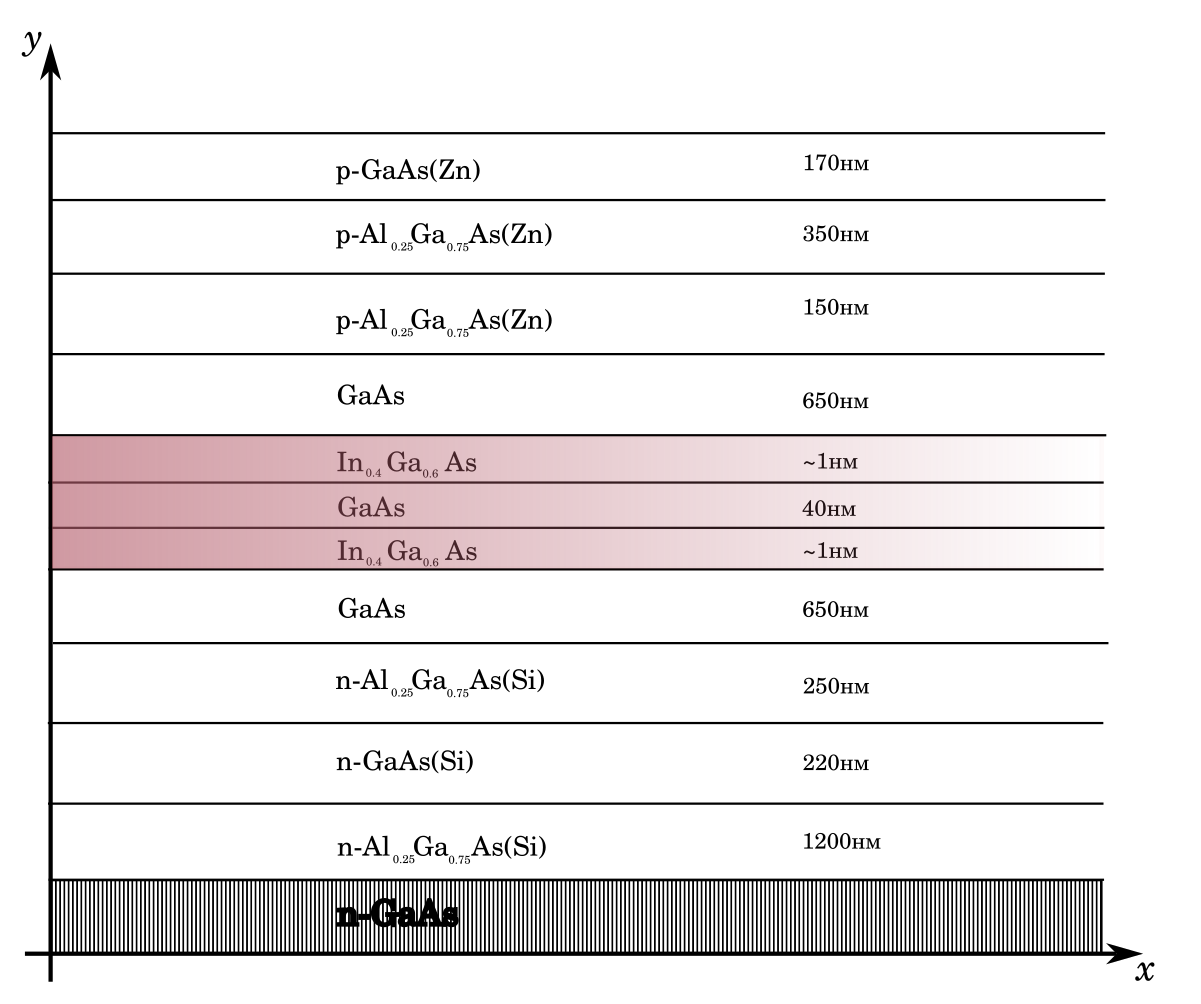
\includegraphics[width=0.59\textwidth]{1.png}
		\caption{Профиль лазера.}
	\end{figure}
	
	\quad В работе предоставлено аналитическое решение уравнения теплопроводности в работающем мощном полупроводниковом лазере. В системе есть два типа источников тепла: нагрев от безызлучательной рекомбинации в активной области и нагрев от омического сопротивления в каждом слое. На подложке GaAs находится плоскость постоянной температуры, которая моделируется как теплоотвод, а на верхнем p-контакте моделируется теплообмен с воздухом комнатной температуры. Левая и правая стенки системы теплоизолированы.
	
	\quad \textit{Аналитическое решение.} Разделим структуру на 9 слоёв с нумерацией от n-AlGaAs(Si) до p-GaAs(Zn). В каждом слое запишем уравнение теплопроводности:
	
	\begin{equation}
		\dfrac{\partial^2 T_i}{\partial x^2} + \dfrac{\partial^2 T_i}{\partial y^2}  = -\dfrac{q_i}{k_i} 
	\end{equation}
	
	\begin{center}
		где $q_i$ — тепловой поток $i$-го слоя, а $k_i$ — теплопроводность $i$-го слоя.
	\end{center}
	
	\quad С условиями непрерывности на границе слоёв:
	
	\begin{equation}
		\begin{cases}
			T_i(x, y)\bigg|_{y=y_i} = T_{i-1}(x, y)\bigg|_{y=y_i} \\
			\dfrac{\partial T_i}{\partial y} \bigg|_{y=y_i} = \dfrac{\partial T_{i-1}}{\partial y}\bigg|_{y=y_i} \\
		\end{cases}
	\end{equation}
	
	
	\quad И граничными условиями: 
	
	\begin{equation}
		\begin{cases}
			\left( k_9\dfrac{\partial T_9}{\partial y} - \alpha T_9\right)\bigg|_{y=h} = -293 \cdot \alpha \\
			T(x, y) \bigg|_{y=0} = 293 \\
			\dfrac{\partial T_i}{\partial x}\bigg|_{x=0,w} = 0 
		\end{cases}
	\end{equation}
	
	\quad Ищем решение в виде суммы частного решения неоднородного уравнения и общего решения однородного уравнения. Разделяя переменные по методу Фурье находим: 
	
	\begin{equation}
		T_i(x, y)  = -\dfrac{q_i }{2k_i} y^2 + C^{(i)}_1 y + C^{(i)}_2 + \displaystyle\sum\limits_{n=1}^{\infty} \left(A^{(i)}_n \sinh{\dfrac{\pi n y}{w}}+ B^{(i)}_n \cosh{\dfrac{\pi n y}{w}} \right) \cos{\dfrac{\pi n x}{w}}
	\end{equation}
	
	\begin{center}
		где: $T_{i, \text{частн.}} =  -\dfrac{q_i }{2k_i} y^2 + C^{(i)}_1 y + C^{(i)}_2$ -  частное решение неоднородной задачи.
		
		$T_{i, \text{общ.}} = \displaystyle\sum\limits_{n=1}^{\infty} \left(A^{(i)}_n \sinh{\dfrac{\pi n y}{w}}+ B^{(i)}_n \cosh{\dfrac{\pi n y}{w}} \right) \cos{\dfrac{\pi n x}{w}}$ - общее решение однородной. 
	\end{center}
	
	\quad Коэффициенты в решении (4) определяются из условий непрерывности (2) и условий на границе слоёв (3). Для каждого из решений (частного неоднородного и общего однородного) можно составить свою систему из 18 уравнений на коэффициенты $C^{(i)}_1$, $C^{(i)}_2$, $A^{(i)}_n$, $B^{(i)}_n$ $\forall n \in \mathbb{N}$. Обе системы уравнений совместны и решаются численно.
	
	\quad \textit{Результаты и выводы.} Полученное выше решение уравнения теплопроводности моделирует температуру в профиле как скалярное поле координат. Значения поля температуры были рассчитаны для тока $I = 10$ А. Полученное распределение показано на рисунке 2. 
	
	\begin{figure}[h!]
		\centering
		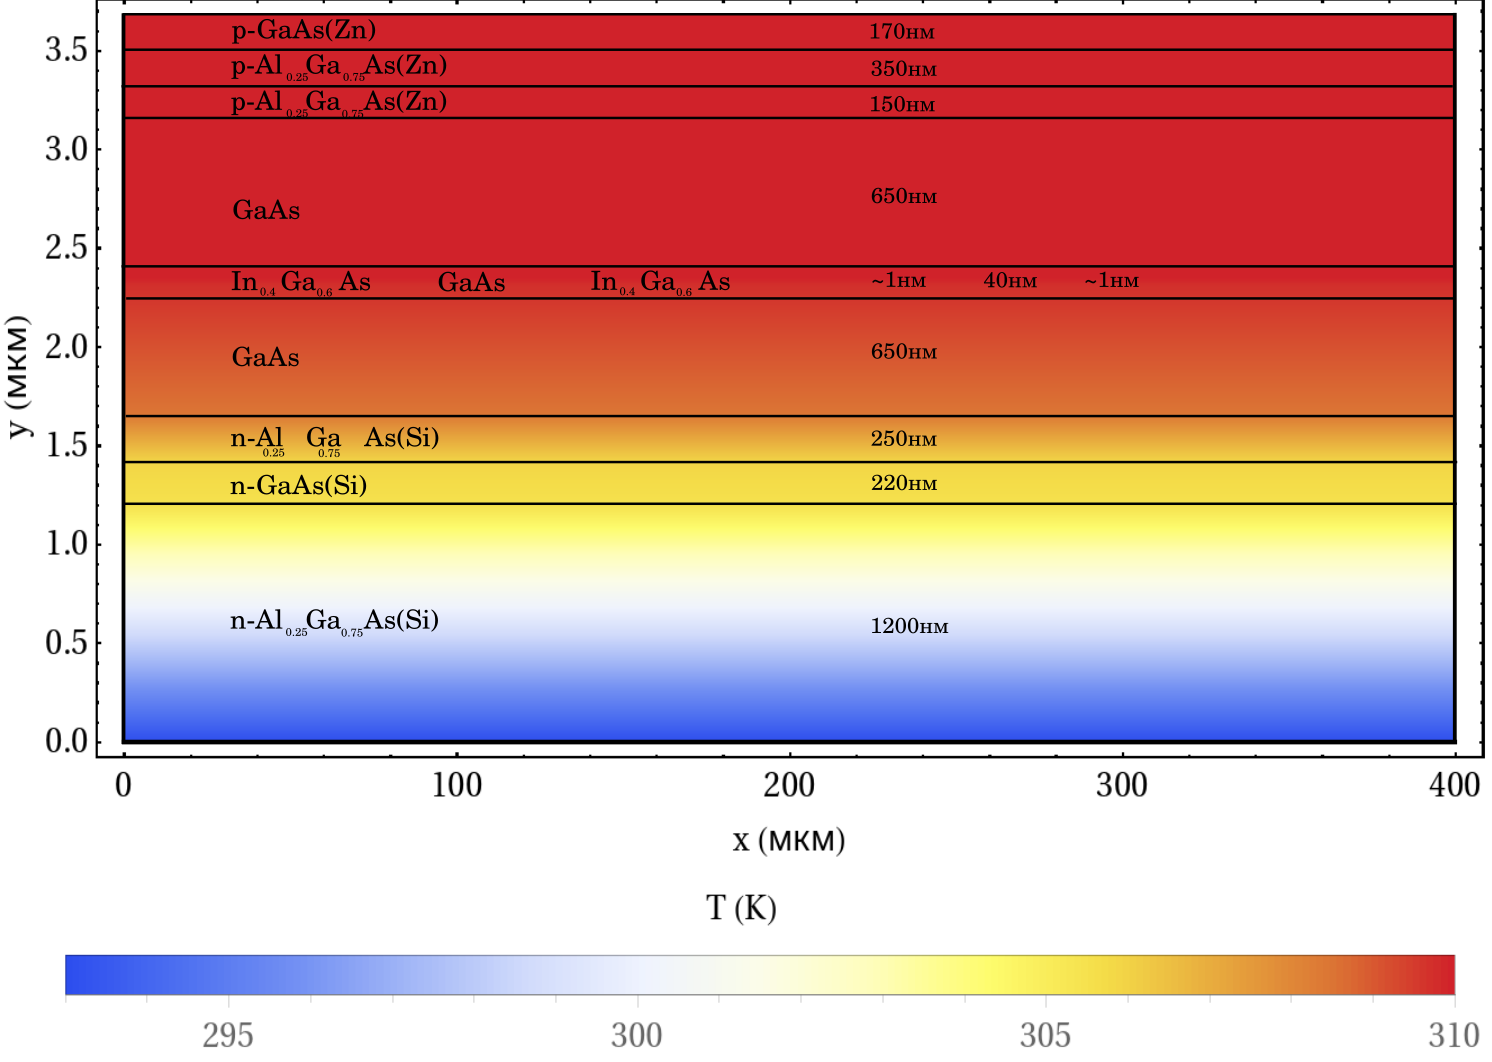
\includegraphics[width=0.8\textwidth]{2_1.png}
		\caption{Распределение температуры в профиле.}
	\end{figure}

	\quad По полученным значениям были сделаны выводы по улучшению теплопроводности гетероструктуры. Так как AlGaAs имеет меньшую теплопроводность по сравнению с GaAs, необходимо уменьшать толщины первого слоя, приближая активную область к теплоотводу
	
	\quad Результаты данного моделирования будут проверены экспериментально для различных толщин и составов слоёв гетероструктуры между активной областью и теплоотводом.
	
	\begin{center}
		ЛИТЕРАТУРА
	\end{center}
	
	1. Afromowitz M.A. Thermal conductivity of Ga$_{1-x}$Al$_{x}$As alloys // Journal of Applied Physics. -- 1973. -- Vol. 44. -- № 3. -- P. 1292-1294.
	
	2. Payusov A.S., Beckman A.A., Kornyshov G.O., Shernyakov Yu.M., Mintairov S.A., Kalyuzhnyy N.A., Kulagina M.M., Maximov M.V., Gordeev N.Yu. Reducing thermal resistance of high-power semiconductor diode lasers with coupled waveguides // Optics \& Laser Technology. -- 2023. -- Vol. 164. -- P. 109484.
	
	3. Кейси Х., Паниш М. Лазеры на гетероструктурах: в 2 т. -- 2-е изд. -- М.: Мир, 1988. -- Т. 2. -- 368 с.
	
	
	1. Формат тезисов поменять, нужен ворд.
	
	2. Добавить нормальную сноску
	
	3. Добавить ссылки на предложения. 
	
	4. Рассказать о том, как посчитаны значения потоков теплопроводности.
	
	Mode Engineering in Lasers Based on Coupled Large Optical Cavities
	
	5. В работе предоставлены аналитические решения и тд. [Кейси Паниш]
	
	
	
\end{document}